\chapter{Introduction}\label{introduction}



An Introduction usually is used only to provide a background, a motivation and a short readers guide. In this document it is used to reproduce some information about writing a thesis and writing in \LaTeX. To get started, just delete this content and start writing your own.

\section{How to Organize your Thesis}
In this section some revision of a generic structure of a thesis will be given. Please note that the complete text can be found on:
\begin{quote}
	http://www.sce.carleton.ca/faculty/chinneck/thesis.html
\end{quote}
Translations to other languages are available too:
\begin{quote}
	http://www.sce.carleton.ca/faculty/chinneck/thesis/translations.html
\end{quote}
Please see also \cite{Leunen:Scholars:1992,Zuber-Skerritt:ThesisWriting:1986}.

\subsection{Introduction}

This is a general introduction to what the thesis is all about -- it is not just a description of the contents of each section. Briefly summarize the question (you will be stating the question in detail later), some of the reasons why it is a worthwhile question, and perhaps give an overview of your main results. This is a birds-eye view of the answers to the main questions answered in the thesis (see above).

\subsection{Background Information (optional)}

A brief section giving background information may be necessary, especially if your work spans two or more traditional fields. That means that your readers may not have any experience with some of the material needed to follow your thesis, so you need to give it to them. A different title than that given above is usually better; e.g., 'A Brief Review of Frammis Algebra.'

\subsection{Review of the State of the Art}

Here you review the state of the art relevant to your thesis. Again, a different title is probably appropriate; e.g., 'State of the Art in Zylon Algorithms.' The idea is to present (critical analysis comes a little bit later) the major ideas in the state of the art right up to, but not including, your own personal brilliant ideas.

You organize this section by idea, and not by author or by publication. For example if there have been three important main approaches to Zylon Algorithms to date, you might organize subsections around these three approaches, if necessary:
\begin{itemize}
	\item[3.1] Iterative Approximation of Zylons
	\item[3.2] Statistical Weighting of Zylons
	\item[3.3] Graph-Theoretic Approaches to Zylon Manipulation
\end{itemize}

\subsection{Research Question or Problem Statement}

Engineering theses tend to refer to a 'problem' to be solved where other disciplines talk in terms of a 'question' to be answered. In either case, this section has three main parts:

\begin{enumerate}
	\item a concise statement of the question that your thesis tackles
	\item justification, by direct reference to section 3, that your question is previously unanswered
	\item discussion of why it is worthwhile to answer this question.
\end{enumerate}

Item 2 above is where you analyze the information which you presented in Section 3. For example, maybe your problem is to 'develop a Zylon algorithm capable of handling very large scale problems in reasonable time' (you would further describe what you mean by 'large scale' and 'reasonable time' in the problem statement). Now in your analysis of the state of the art you would show how each class of current approaches fails (i.e. can handle only small problems, or takes too much time). In the last part of this section you would explain why having a large-scale fast Zylon algorithm is useful; e.g., by describing applications where it can be used.

Since this is one of the sections that the readers are definitely looking for, highlight it by using the word 'problem' or 'question' in the title: e.g. 'Research Question' or 'Problem Statement', or maybe something more specific such as 'The Large-Scale Zylon Algorithm Problem.'

\subsection{Description of How You Solved the Problem or Answered the Question}

This part of the thesis is much more free-form. It may have one or several sections and subsections. But it all has only one purpose: to convince the examiners that you answered the question or solved the problem that you set for yourself in Section 4. So show what you did that is relevant to answering the question or solving the problem: if there were blind alleys and dead ends, do not include these, unless specifically relevant to the demonstration that you answered the thesis question.

\subsection{Conclusions}

You generally cover three things in the Conclusions section, and each of these usually merits a separate subsection:

\begin{enumerate}
	\item Conclusions
	\item Summary of Contributions
	\item Future Research
\end{enumerate}

Conclusions are not a rambling summary of the thesis: they are short, concise statements of the inferences that you have made because of your work. It helps to organize these as short numbered paragraphs, ordered from most to least important. All conclusions should be directly related to the research question stated in Section 4. Examples:

\begin{enumerate}
	\item The problem stated in Section 4 has been solved: as shown in Sections ? to ??, an algorithm capable of handling large-scale Zylon problems in reasonable time has been developed.
	\item The principal mechanism needed in the improved Zylon algorithm is the Grooty mechanism.
	\item Etc.
\end{enumerate}

The Summary of Contributions will be much sought and carefully read by the examiners. Here you list the contributions of new knowledge that your thesis makes. Of course, the thesis itself must substantiate any claims made here. There is often some overlap with the Conclusions, but that's okay. Concise numbered paragraphs are again best. Organize from most to least important. Examples:

\begin{enumerate}
	\item Developed a much quicker algorithm for large-scale Zylon problems.
	\item Demonstrated the first use of the Grooty mechanism for Zylon calculations.
	\item Etc.
\end{enumerate}

The Future Research subsection is included so that researchers picking up this work in future have the benefit of the ideas that you generated while you were working on the project. Again, concise numbered paragraphs are usually best. 

\subsection{Appendices}

What goes in the appendices? Any material which impedes the smooth development of your presentation, but which is important to justify the results of a thesis. Generally it is material that is of too nitty-gritty a level of detail for inclusion in the main body of the thesis, but which should be available for perusal by the examiners to convince them sufficiently. Examples include program listings, immense tables of data, lengthy mathematical proofs or derivations, etc. 

\subsection{Bibliography}

The list of references is closely tied to the review of the state of the art given in section 3. Most examiners scan your list of references looking for the important works in the field, so make sure they are listed and referred to in section 3. Truth be known, most examiners also look for their own publications if they are in the topic area of the thesis, so list these too. Besides, reading your examiner's papers usually gives you a clue as to the type of questions they are likely to ask.

All references given must be referred to in the main body of the thesis. Note the difference from a Bibliography, which may include works that are not directly referenced in the thesis. Organize the list of references either alphabetically by author surname (preferred), or by order of citation in the thesis. 



\section{Revision: Writing in \LaTeX}
As thought in the seminars, \LaTeX is quite useful for writing a paper or a thesis. Nevertheless it comes with its own rules.

\subsection{Word processing with \LaTeX}
\label{sec:model:subsec:latex}

This document has already introduced the most important constructs of
\LaTeX. What is necessary to produce documents with \LaTeX is simple
any normal text editor and a \LaTeX distribution. This is commonly
installed on practically all UNIX-type systems; for Windows, an
excellent \LaTeX exists, called MikTeX, available from
\url{www.miktex.org}. Almost all distributions come with a large patch
of examples and introductory material; consult your local installation
for details. 

Lots of supplementary and background information, FAQs, etc.\ is
available from the Comprehensive TeX Archive Network (CTAN); the
German mirror of which is \url{www.dante.de}. 

\subsection{Tables in \LaTeX}
\label{sec:model:subsec:tables}
The table should be centred and should always have a caption positioned above it. A caption in a sentence form as well as in a short form must end with a period as seen in table~\ref{tab:sample}. Ideally the table can be understood sorely by the table and the caption itself. The parameters ``hbtp'' provide a list of priorities for the arrangement of the table: here, bottom, top, (next) page.

\begin{table}[hbtp]
  \caption{This caption has one line so it is centered.}\label{tab:sample} 
  \centering
  \begin{tabular}{|c|c|}
    \hline
    Example column 1 & Example column 2 \\
    \hline
    Example text 1 & Example text 2 \\
    \hline
  \end{tabular}
\end{table}

\subsection{Figures in \LaTeX}
\label{sec:model:subsec:figures}
Note that a figure is a so-called floating object: it is moved around the actual text in order to best fit on a page. This is in strong contrast to some GUI-based word processing tools, where the placement of figures is usually more associated with luck than principle.

As figures float around, expressions like ``the following figure'' must never be used. Instead, figures need a caption, a label, and must be properly referenced in the main text. A figure caption is placed centred below the figure and describes the figure in (very) short. Again, ideally the figure can be understood sorely by the figure and the caption itself.

In general, only vector graphics in encapsulated postscript (EPS) or a similar format (SVG, PDF) should be included in any kind of text, as this allows arbitrary scaling, rotation etc.\ without any loss of quality. Bitmap formats (JPEG, GIF, \dots) should only be used if no other alternative exists --- basically the only case where bitmaps can be justified is when scanned pictures need to be included in a text, however, this should be avoided as hard as possible as the quality in usually not satisfactory. If a screen shot is needed a high resolution picture without visible fragments of a jpeg compression is allowed. Figures like the figure~\ref{fig:samplefig} (this is how you refer to figures correctly! the tilde is used as a non-breaking space) should always appear after the first referencing it.
\begin{figure}[hbtp]
	 \centerline{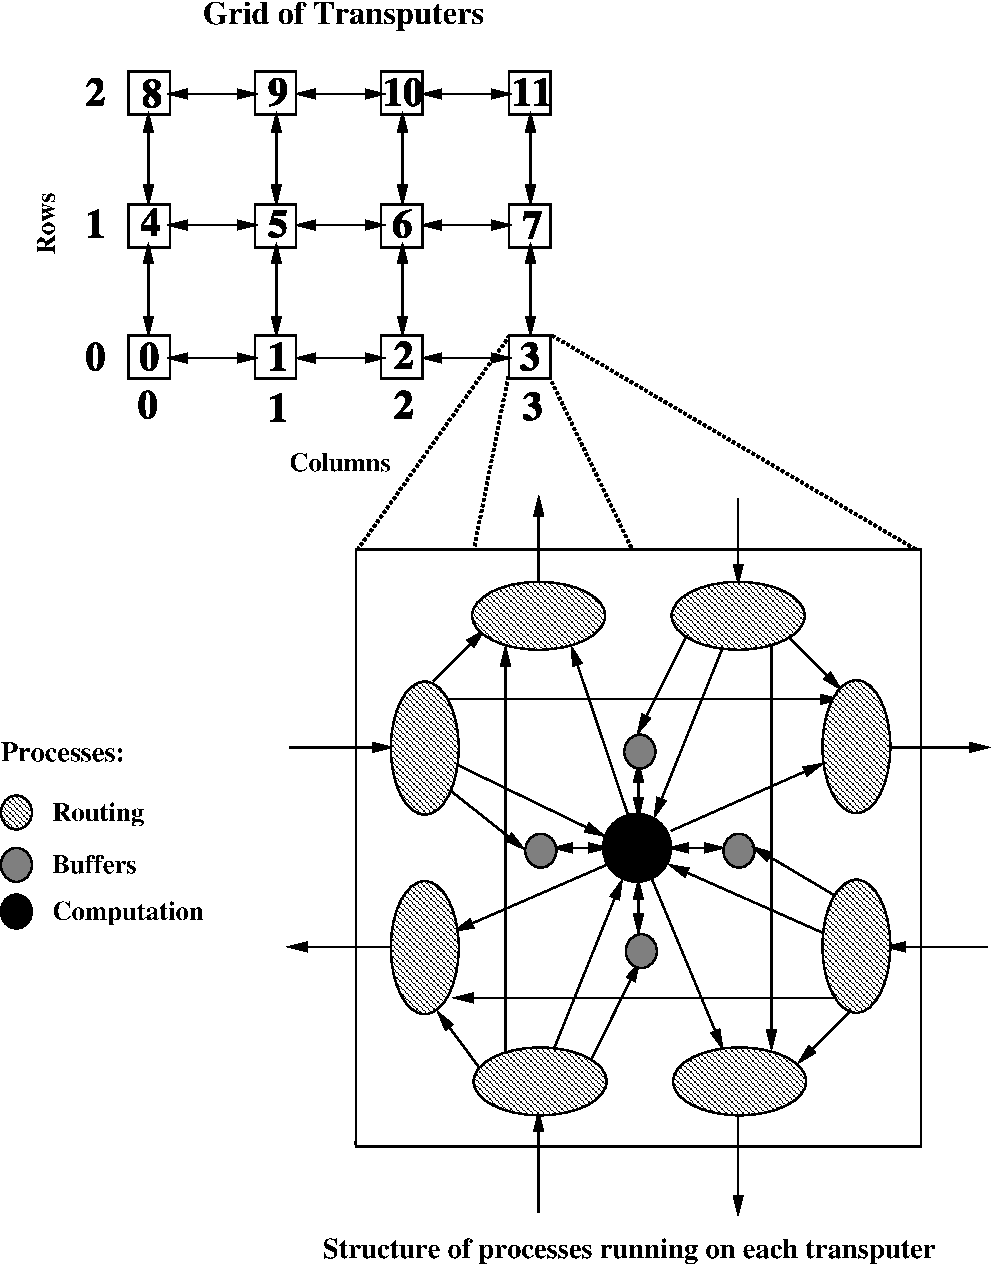
\includegraphics[width=0.6\textwidth]{samplefig.pdf}}
	 {\caption{Network of transputers and the structure of individual
processes.}\label{fig:samplefig}}
\end{figure}